% Options for packages loaded elsewhere
\PassOptionsToPackage{unicode}{hyperref}
\PassOptionsToPackage{hyphens}{url}
%
\documentclass[
]{article}
\usepackage{lmodern}
\usepackage{amssymb,amsmath}
\usepackage{ifxetex,ifluatex}
\ifnum 0\ifxetex 1\fi\ifluatex 1\fi=0 % if pdftex
  \usepackage[T1]{fontenc}
  \usepackage[utf8]{inputenc}
  \usepackage{textcomp} % provide euro and other symbols
\else % if luatex or xetex
  \usepackage{unicode-math}
  \defaultfontfeatures{Scale=MatchLowercase}
  \defaultfontfeatures[\rmfamily]{Ligatures=TeX,Scale=1}
\fi
% Use upquote if available, for straight quotes in verbatim environments
\IfFileExists{upquote.sty}{\usepackage{upquote}}{}
\IfFileExists{microtype.sty}{% use microtype if available
  \usepackage[]{microtype}
  \UseMicrotypeSet[protrusion]{basicmath} % disable protrusion for tt fonts
}{}
\makeatletter
\@ifundefined{KOMAClassName}{% if non-KOMA class
  \IfFileExists{parskip.sty}{%
    \usepackage{parskip}
  }{% else
    \setlength{\parindent}{0pt}
    \setlength{\parskip}{6pt plus 2pt minus 1pt}}
}{% if KOMA class
  \KOMAoptions{parskip=half}}
\makeatother
\usepackage{xcolor}
\IfFileExists{xurl.sty}{\usepackage{xurl}}{} % add URL line breaks if available
\IfFileExists{bookmark.sty}{\usepackage{bookmark}}{\usepackage{hyperref}}
\hypersetup{
  pdftitle={Optimal Stopping Problem - PSET},
  pdfauthor={Jake Underland},
  hidelinks,
  pdfcreator={LaTeX via pandoc}}
\urlstyle{same} % disable monospaced font for URLs
\usepackage[margin=1in]{geometry}
\usepackage{graphicx,grffile}
\makeatletter
\def\maxwidth{\ifdim\Gin@nat@width>\linewidth\linewidth\else\Gin@nat@width\fi}
\def\maxheight{\ifdim\Gin@nat@height>\textheight\textheight\else\Gin@nat@height\fi}
\makeatother
% Scale images if necessary, so that they will not overflow the page
% margins by default, and it is still possible to overwrite the defaults
% using explicit options in \includegraphics[width, height, ...]{}
\setkeys{Gin}{width=\maxwidth,height=\maxheight,keepaspectratio}
% Set default figure placement to htbp
\makeatletter
\def\fps@figure{htbp}
\makeatother
\setlength{\emergencystretch}{3em} % prevent overfull lines
\providecommand{\tightlist}{%
  \setlength{\itemsep}{0pt}\setlength{\parskip}{0pt}}
\setcounter{secnumdepth}{-\maxdimen} % remove section numbering
\usepackage{amsmath}
\usepackage{dcolumn}
\usepackage{rotating}
\usepackage{bbm}
\usepackage{setspace}
\usepackage{hyperref}
\usepackage{amsmath}
\usepackage{dcolumn}
\usepackage{rotating}
\usepackage{hyperref}

\title{Optimal Stopping Problem - PSET}
\usepackage{etoolbox}
\makeatletter
\providecommand{\subtitle}[1]{% add subtitle to \maketitle
  \apptocmd{\@title}{\par {\large #1 \par}}{}{}
}
\makeatother
\subtitle{Topics in Macroeconomics: DSGE Models (Fall, 2021/22)}
\author{Jake Underland}
\date{2022/02/01}

\begin{document}
\maketitle

{
\setcounter{tocdepth}{2}
\tableofcontents
}
Think about the investment model in the lecture. In this report, you
will numerically solve this model using the value function iteration
method with Matlab. We derived some equations in the lecture, but in
this report you can use only two functions below.\\

\begin{itemize} 
\item Value function: $V(z)=\max\left\{ \beta \int_0^B V(z')dF(z'), z - I \right\}$
\item Policy function: $\begin{cases} \text{invest} \;\;\; \text{if } z > z^* \\\text{wait} \;\;\:\:\: \text{ if } z \le z^*\end{cases}$
\end{itemize}

Parameter values and the shape of distribution \(F(z)\) are up to you.

\hypertarget{problem-1}{%
\section{Problem 1}\label{problem-1}}

\textbf{Question 1}: Solve this problem using the value function
iteration method. You need to discretize \(V(z)\) and \(F(z)\) on a
finite number of grids. Also, use the initial guess of the value
function as \(V (z) = 0\) for all \(z\). Plot \(V (z)\) and discuss its
shape. \[\dagger\] For this first exercise, I used the following
parameters: \[
\begin{aligned}
\beta &= 0.98 \\
I &= 2 \\
F &\sim Unif\left[0, 5\right]
\end{aligned}
\] The high discount factor \(\beta\) suggests that our investor is
patient and is willing to wait to increase their profits. Furthermore,
the cost of \(I = 2\) for investment means that any value between 2 and
5 will yield a profit, and since the distribution is uniform, the
expected value of returns will be considerably higher than the cost.
Judging from all the above, we can expect the cutoff value for the
policy function \(z^*\) will be quite high. Below, I plot the optimized
value function \(V(z)\).

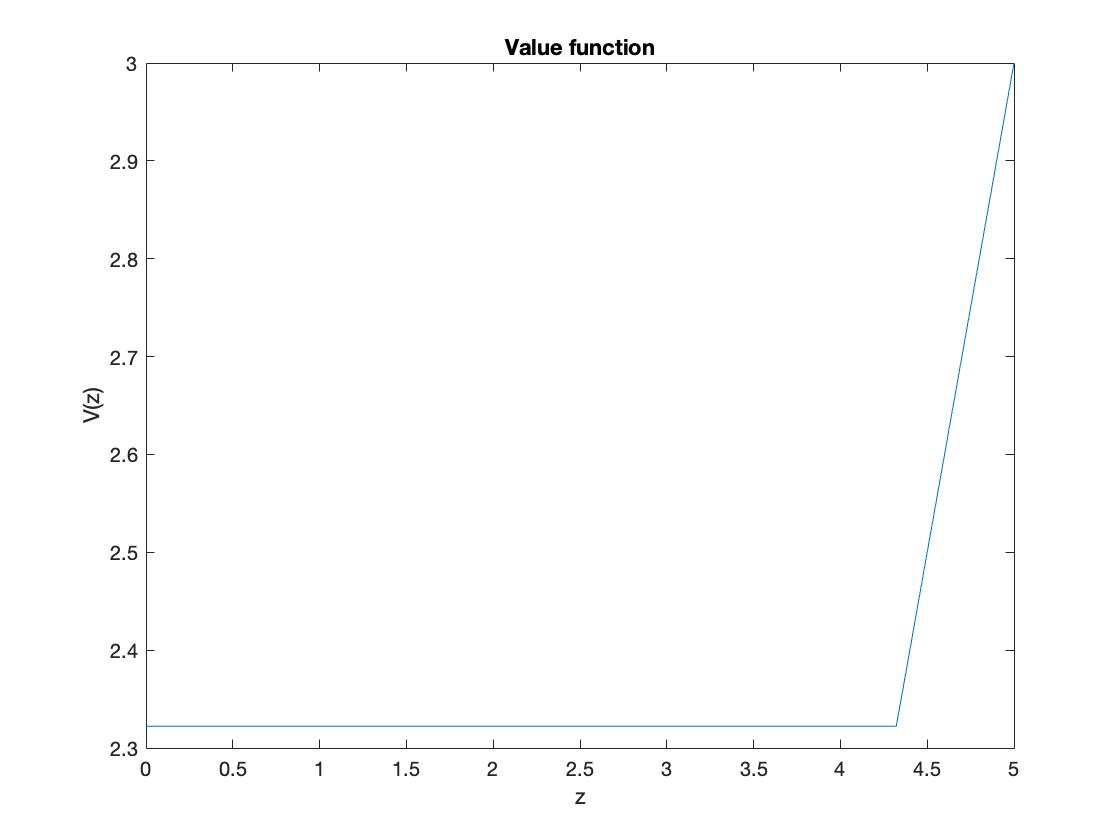
\includegraphics{images/valfunc1.jpg}

The graph tells us that the cutoff value \(z^* \approx 4.32\) and the
corresponding \(V(z^*) \approx 2.32\). As we expected, the cutoff value
is quite high and shows that the investor is well posed to wait for a
favorable outcome. The graph is flat until \(z = z^*\), meaning the
investor will wait for any value below the cutoff value, and hence their
utility will be the expected utility of waiting, which is \(V(z^*)\).
Above the cutoff value, the investor will take any offer and pay the
cost, keeping the difference as a profit.

\hypertarget{problem-2}{%
\section{Problem 2}\label{problem-2}}

\textbf{Question 2}: Change the parameter values of \(I\) and \(\beta\).
Plot \(V (z)\) and discuss how and why the shape is changed. \[\dagger\]
Now, we change the parameters as below: \[
\begin{aligned}
\beta &= 0.7 \\
I &= 1 \\
\end{aligned}
\]

We will use the same distribution of \(z\).\\
Now, we have an impatient investor with a discount factor of \(0.7\),
meaning they are less willing to wait to invest and prefer a moderate
immediate profit to a high profit in the distant future. On the other
hand, now the investor has a cost of investment of only \(I = 1\),
suggesting it is much easier for them to make a profit from the
investment. This may also induce the investor to take a lower cutoff
value, since they would require less to make a considerable profit off
of the investment. We plot \(V(z)\) with these renewed parameters below:

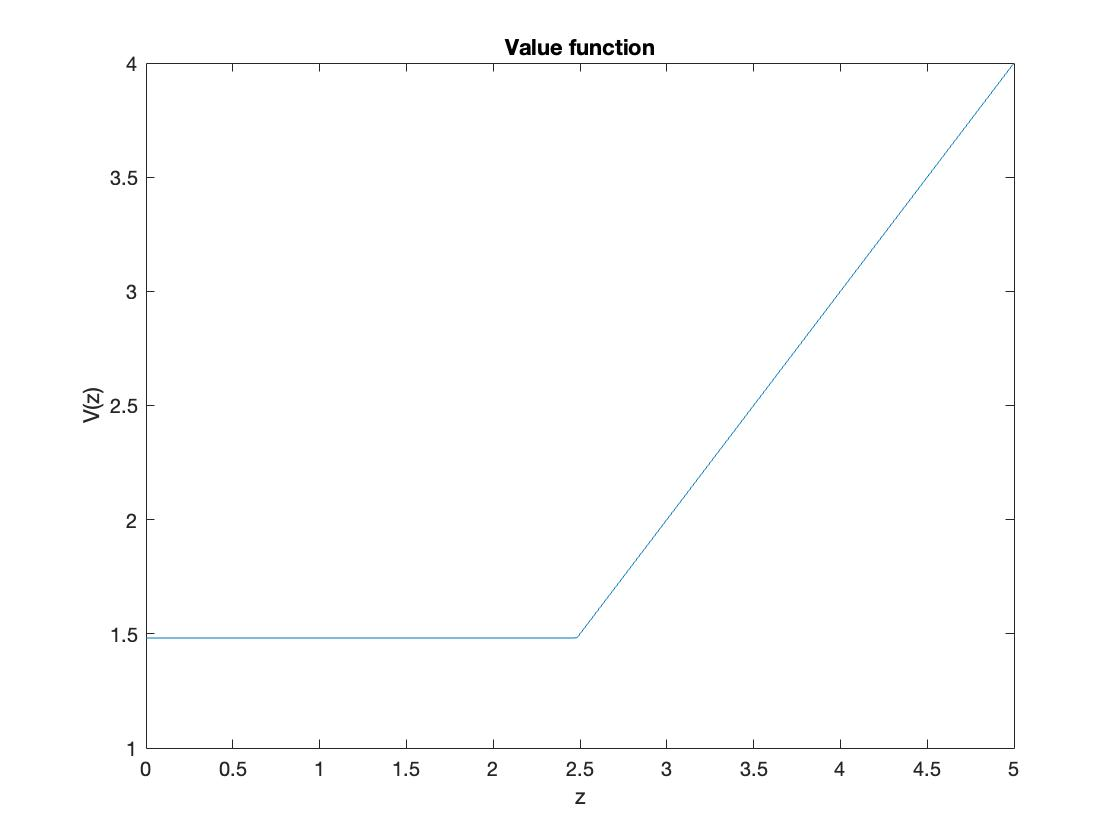
\includegraphics{images/valfunc2.jpg} As we expected, the cutoff value
is now \(z^* \approx 2.48\) and \(V(z^*) \approx 1.48\). This confirms
our prediction that the cutoff value would be considerably lower than in
problem 1, and our new investor would be much more eager to sell their
investment at an earlier time.

\hypertarget{problem-3}{%
\section{Problem 3}\label{problem-3}}

\textbf{Question 3}: Suppose that the investor can get two investment
opportunities each period. These follow the same distribution as in
Question 1. In addition, these two are independent. Each period, the
investor can take the better offer, or wait. Solve this problem using
the value function iteration method. Plot \(V (z)\) and compare the
result with Question 1. \[\dagger\] Let the returns from the two
investment opportunities be random variables
\(Z_1, Z_2 \stackrel{i.i.d.}{\sim} Unif[0, 5]\). Then, we know that at
every investment opportunity, the investor would invest in
\(\max\{Z_1, Z_2\}\). Consider the following:\\
\newline Assume there are two uniform random variables
\(X_1, X_2 \stackrel{i.i.d.}{\sim} Unif[a, b]\). Then, we consider the
distribution of \(Z = \max \{X_1, X_2\}\). \[\begin{aligned}
F_Z(z) &= F_{X_1}(z) F_{X_2}(z) \\
&= \left(\frac{z - a}{b - a}\right)^2 \\
f_Z(z) &= \frac{\partial}{\partial z} \left(\frac{z - a}{b - a}\right)^2 \\
&= \frac{2(z-a)}{(b-a)^2}
\end{aligned}\] \newline Therefore, we can treat the two independent
investment opportunities as one random variable. Then, we plug in the
upper and lower bound values to the probability distribution function of
two iid uniform variables we have derived above. If we denote
\(Z = \max\{Z_1, Z_2\}\), and the pdf of \(Z\) as \(f_Z\), then
\[f_Z(z) = \frac{2z}{25}\] Therefore, the problem now is restated as
finding the optimal cutoff point for an investment opportunity \(Z\)
which has a probability distribution function of
\(f_Z(z) = \frac{2z}{25}\). In order to approximate this probability
density function to probability mass function in our discrete
representation of \(z\), we instead use
\(f_Z(z_i) \approx F_Z(z_i) - F_Z(z_{i-1})\). Then, using the same
parameters as in question 1, we get the following graph:\\
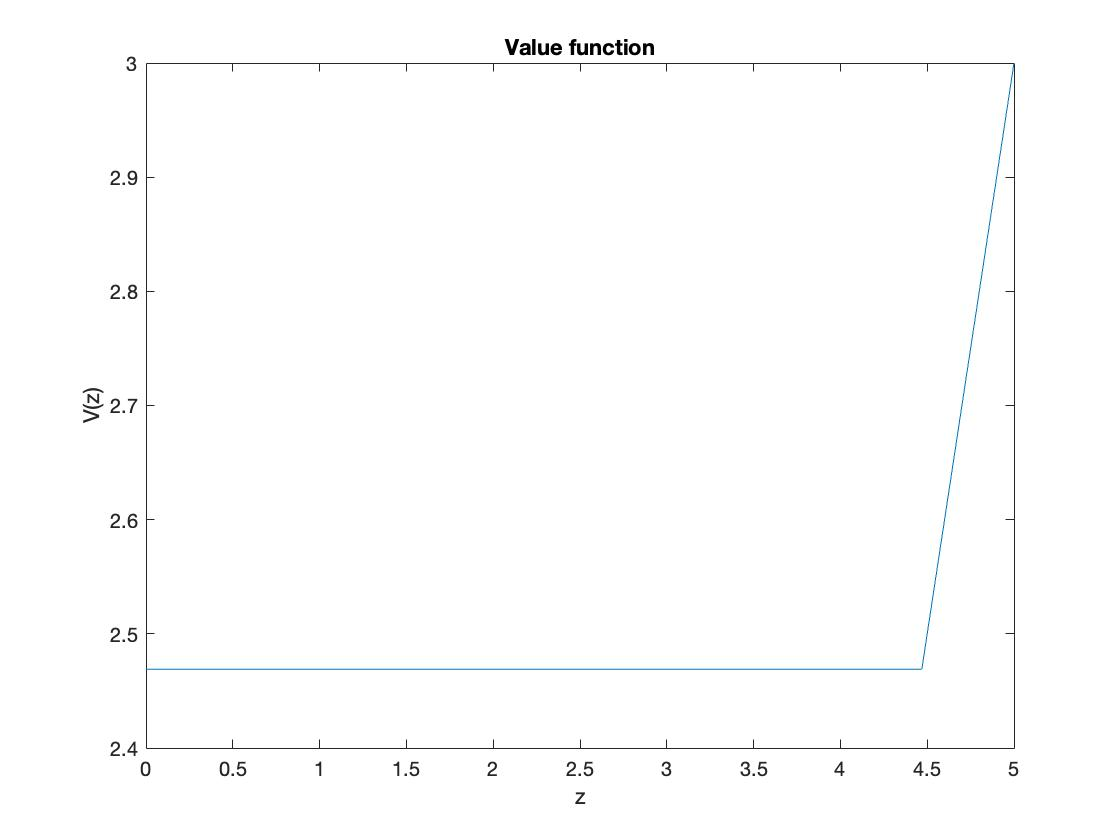
\includegraphics{images/valfunc3.jpg} Now, the cutoff point \(z^*\) has
increased from its value of \(4.32\) in question 1 to \(4.46\) in
question 4. Concomitantly, the value function \(V(z^*)=2.46\). The
reason for this increase is that the new distribution renders larger
values of \(z\) more probable than lower values of \(z\), a direct
result of using the maximum function on two identically distributed
independent variables.

\hypertarget{problem-4}{%
\section{Problem 4}\label{problem-4}}

\textbf{Question 4}: This investment model is an example of optimal
stopping problem. In the lecture, I talked about job search as another
example. Provide one more example of the optimal stopping problems from
your daily life or experience. Describe your story and discuss the
similarity with the optimal stopping problem. Then, write down your
story as a mathematical model. Give reasonable parameter values, and
solve it using Matlab. Then, plot the diagrams and discuss your results.
Finally, change some parameter values and discuss its implications.
\[\dagger\] Dating, in many ways, is an optimal stopping problem. For
many people, dating is a means for them to search viable candidates for
them to marry and, perhaps, raise a family with. Therefore, it might be
reasonable to assume that people are appraising each of their romantic
partners in order to marry the optimal one. Let us assume just that,
that people date to find one person that they will marry, and that they
do not derive utility solely from the act of dating itself. Furthermore,
let us also assume that there is a cost to knowing the ``quality'' of a
person, whether they will make a good spouse or not. This is the cost of
actually dating them. We also take into consideration the fact that
people often prefer to get married before a certain age (which can be
convenient if one has plans of having children), and so there would
exist a discount factor for waiting on the decision to marry a partner.
Finally, we assume that prospective partners come distributed according
to a normal distribution, where most partners are of average appeal to
the individual, and some are particularly desirable or particularly
undesirable.\\
Factoring in all of the above, we get a problem identical to the optimal
stopping problem we have solved above. Let the cost of knowing a person
be \(I\), the discount factor for waiting on marriage be \(\beta\), and
the ``quality'' of a partner be
\(Z \sim N\left(5, (\frac{5}{3})^2\right)\). This is making use of the
nifty characteristic of the normal distribution that the normal 99\% of
all normally distributed data lies within \(\mu \pm 3\sigma\). What this
means for us is the oft seen 1\textasciitilde10 ranking system of
romantic partners. Not that I condone of such a reductive scale for
measuring humans, but for the sake of expediency, this is what we will
use in this exercise. In summary, we can formulate the problem as thus:

\begin{itemize} 
\item Value function: $V(z)=\max\left\{ \beta \int_0^B V(z')dF(z'), z - I \right\}$
\item Policy function: $\begin{cases} \text{marry} \;\;\; \text{if } z > z^* \\\text{wait} \;\;\;\;\: \text{ if } z \le z^*\end{cases}$
\end{itemize}

where \[\begin{aligned} F&\sim N(5, (\frac{5}{3})^2)\end{aligned}\]
First, we will assume a young individual in the dating scene. For young
people, there is plenty of time for them to search the market before
settling down, so it is reasonable to expect their discount factor
\(\beta\) to be quite high. Furthermore, considering that dating is
often a time intensive activity, for young people who generally tend to
have lower income and more time on their hands, the opportunity cost of
dating is also low, making \(I\) low as well. For these reasons, we will
assume the following parameter values: \[\begin{aligned} \beta&= 0.99\\
I &= 0.5
\end{aligned}\] With these values we get the following distribution for
the value function\\
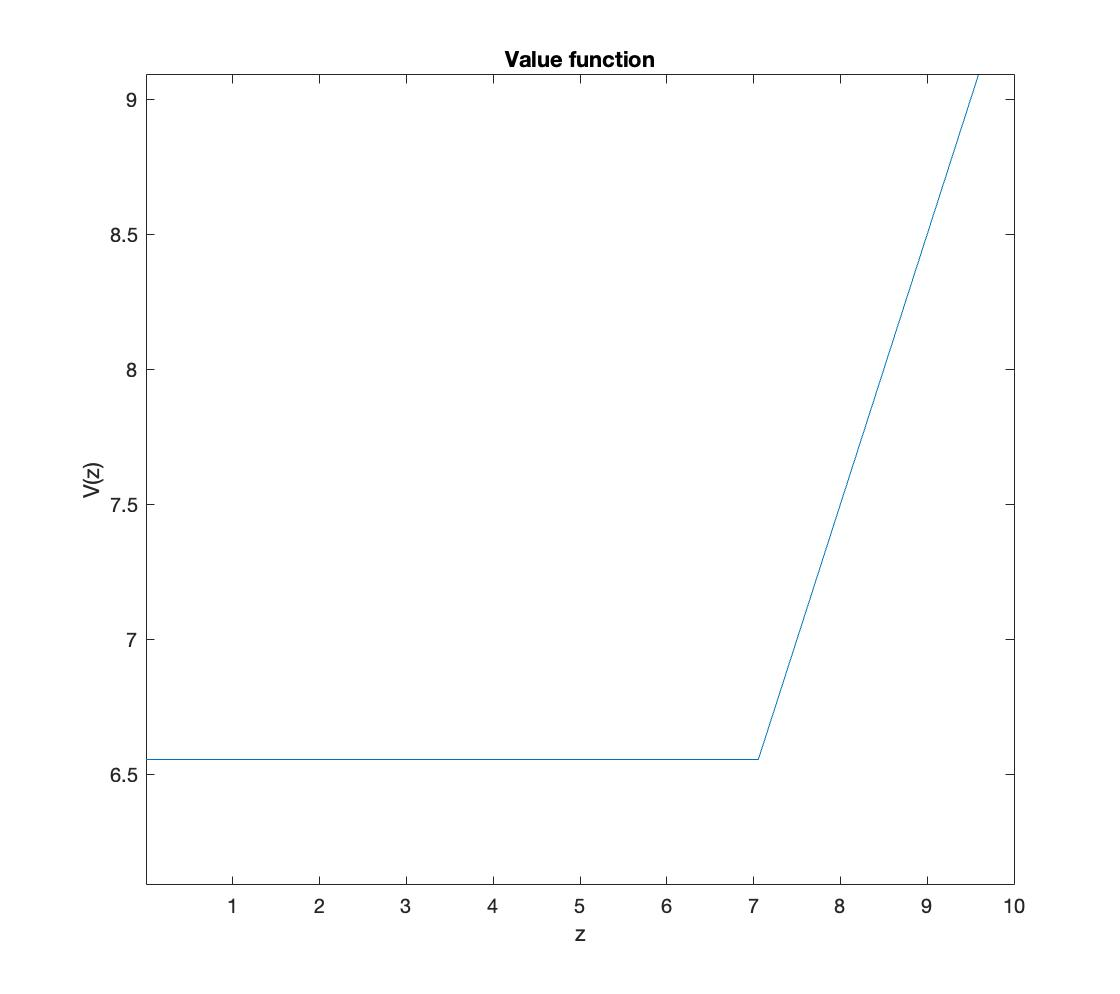
\includegraphics{images/datingvalfunc.jpg} The cutoff value in the above
graph is \(z^* = 7.05\). This shows us that for a young person, the
optimal strategy is to keep waiting for a person of relatively high
appeal before settling down to marry.\\
Next, we consider an older individual in the dating market. For an older
individual who wants children, waiting for another partner and delaying
marriage comes with a much greater cost. Furthermore, because older
people are more likely to have higher income and also be busier than
younger people, this individual's opportunity cost for dating,
i.e.~\(I\) in our model, is expected to be much higher than the younger
individual. Let us assign \[\begin{aligned} \beta&= 0.6\\
I &= 3
\end{aligned}\] The lower \(\beta\) would suggest this individual would
be more eager to marry a partner, whereas a higher \(I\) would imply the
opposite, that is, the individual would want to wait for a more
appealing partner in order to fully compensate for the cost of dating
and knowing them. We graph the value function below:\\
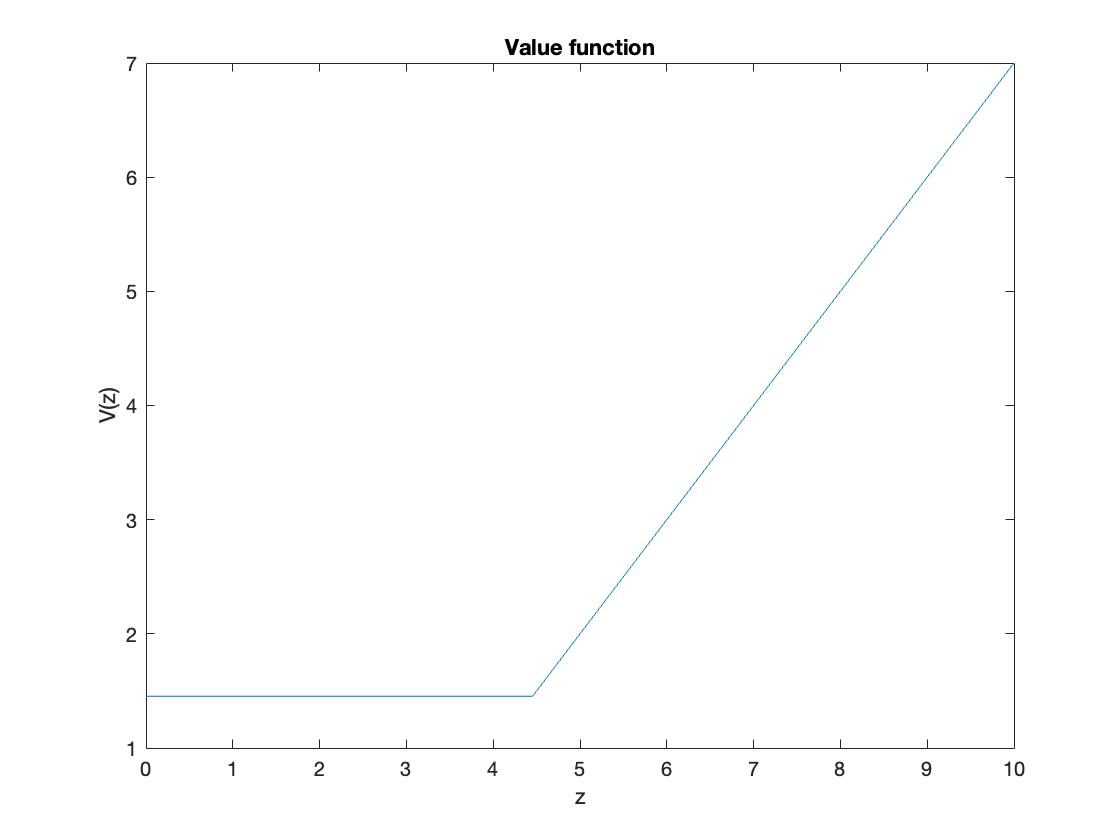
\includegraphics{images/olderdatingvalfunc.jpg} The cutoff point is now
\(z^* = 4.45\), and the profit \(V(z^*) = 3.45\). The effect of a much
smaller \(\beta\) is prominent in this case, as the individual is far
more eager to marry than the younger individual we examined earlier.\\
Until now, we have assumed that although there was an element of
randomness in a partner's desirability, once a desirable candidate was
found, marriage was a definite option for the individual. However, more
realistically, we can say that the more desirable a romantic partner is,
the less likely it will be to get them to marry you. That's why, in this
final section I change the distribution of partners. Let
\(Z \sim \left(0, (\frac{10}{3})^2\right)\). But, we want this to be an
asymmetric distribution, since we want all our values positive and most
to lie between 0 and 10. \[\begin{aligned} 
Z &\sim N\left(0, (\frac{10}{3})^2\right)  \implies \frac{Z^2}{100 / 9} \sim \chi^2_1 \\
\implies Z^2 &= \frac{100}{9}\chi^2_1 = Gamma(1/2, 200 / 9)\\
\end{aligned}\] This way, the individual has a higher chance of being
able to date a partner that is undesirable, but a much lower chance of
dating someone with higher desirability. We simulate this model with the
same parameters as our young romantic and observe what it does to the
cutoff value.\\
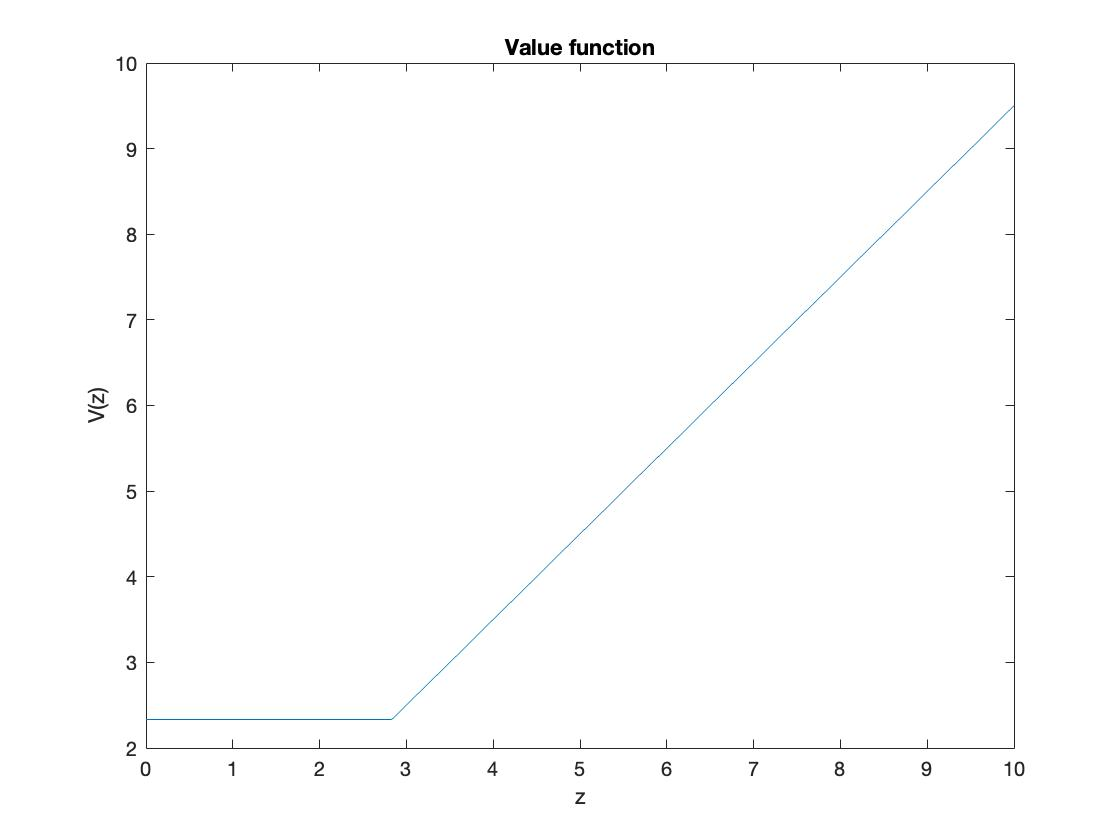
\includegraphics{images/realisticdating.jpg} The new threshold for
marriage is an astonishing \(z^* \approx 2.83\). Maybe we have
underestimated the charm of this individual a bit too much, and could
have found a more appropriate right-skewed distribution to fit their
chance of success. However, the tragic fact remains: if you want an
optimal marriage, you need to first increase your own desirability to
improve your chances of success in dating.\\
An interesting insight gained from this exercise is that if we are able
to appropriately measure our success rate at proposing to prospective
spouses, we might be able to formulate an optimal choice policy for who
to marry to maximize our utility. Seems a bit cold, but efficient.

\end{document}
